\documentclass[9pt, compress]{beamer}
\usetheme[titleprogressbar]{m}

\usepackage[scale=2]{ccicons}
\usepackage{minted}
\usepackage{booktabs}
\usepackage{multirow}
\usepackage{amsmath}
\usepackage{arydshln}
\usepackage{amssymb}
\usepgfplotslibrary{dateplot}
\usepackage{booktabs,caption,fixltx2e}
\usepackage[flushleft]{threeparttable}
\usepackage{color}


\usepackage{tikz}
\usepackage{verbatim}
\usetikzlibrary{arrows,positioning,calc} 
\usepackage{relsize}
\newcommand\LM{\ensuremath{\mathit{LM}}}
\newcommand\IS{\ensuremath{\mathit{IS}}}

\tikzset{
    %Define standard arrow tip
    >=stealth',
    %Define style for boxes
    punkt/.style={
           rectangle,
           rounded corners,
           draw=black, very thick,
           text width=6.5em,
           minimum height=2em,
           text centered},
    % Define arrow style
    pil/.style={
           <-,
           thick,
           shorten <=2pt,
           shorten >=2pt,},
    % Node for explanation       
    punk/.style={
           rectangle,
           draw=white, thin,
           text width=17em,
           minimum height=2em,
           text centered}   
}
\usepackage{pgfplots}

\author{Syngjoo Choi (SNU), Booyuel Kim (KDIS), Minseon Park (KDI), Yoonsoo Park (KDI), and Euncheol Shin (KHU)} 
\title{Rationality, Preference Aggregation and Pareto Efficiency of Group Decision Under Risk}
%\subtitle{}
%\logo{}
%\institute{\textbf{KDI}}
\date{June 13th, 2017}
%\subject{}
%\setbeamercovered{transparent}
%\setbeamertemplate{navigation symbols}{}
\begin{document}
	\maketitle
    \begin{frame}\frametitle{Introduction}
	\begin{itemize}
    \item We make many types of collective decision in our daily life
    \begin{itemize}
    \item Household's decision on consumption and saving, a firm's  resource allocation among projects, decision on tax and transfer in legislature
    \end{itemize}
    \item The central challenge is individuals within a collective usually have different preferences, especially over the risk
     \item This led much investigations on how individuals' different risk preferences are aggregated (Baillon et al. (2016), Bateman and Munro (2005), Palma et al. (2010))
    \item There also exist a bunch of studies on the consistency of group decision especially when such aggregation is not successful (Arrow (1951), Browning and Chiappori (1998), Chiappori and Ekeland (2011), Bourguignon et al. (2009))
    \end{itemize}
    \end{frame}
   
    \begin{frame}\frametitle{Fundamental Questions on Group Decision}
    Three fundamental questions on group decision
    \begin{block}{1. Rationality Extension:}
    If each individual's choices are consistent with the utility maximization model, are group's choices also be? 
    \end{block}
    \begin{block}{2. Risk Preference Aggregation:}
    Are individuals' risk preferences reflected into that of a group?
    \end{block}
    \begin{block}{3. Pareto Efficiency:}
    Are group's choices Pareto efficient? Are they maximizing the social welfare?
    \end{block}
	\end{frame}
    
	\begin{frame}\frametitle{Contribution}
    Our contribution is that using a unique experimental design and a large data set, we answer such fundamental questions, factors for these properties, and the relationship among them 
    \begin{enumerate}    
    \item Taking the revealed preference approach, we investigate the relationship between individual and group rationality 
    \item We devise a novel way to test Pareto efficiency given individual and collective choice data 
    \item We collected rich (demographic variables, cognitive ability, network, personality) and large (N=1572) data set, which enriches the analysis 
    \end{enumerate}
    \end{frame}
    
    \begin{frame}\frametitle{Experimental Design and Procedures}
    \label{decision}
        \begin{itemize}
        \item Our decision environment is based on Choi et al. (2007) 
        \item There are two states $\lbrace 1,2 \rbrace$ which occur randomly and equally likely ($p(S=1)=p(S=2)=0.5$)
        \item A subject chooses the combination \((x_1,x_2)\) on the given budget line \(p_1x_1+p_2x_2=1\) 
        \item The subject receives the points $x_1$ if the state is $1$, and $x_2$ in the other case
        \end{itemize}
\begin{center}        
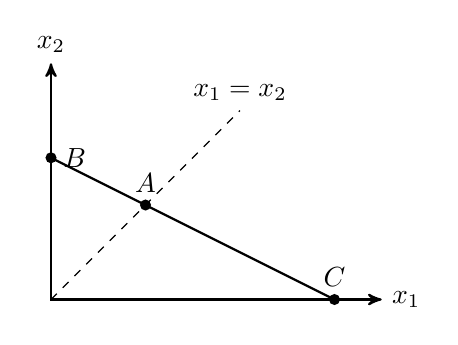
\begin{tikzpicture}[
        scale=1.2,
        IS/.style={black, thick},
        LM/.style={black, dashed},
        axis/.style={thick, ->, >=stealth', line join=miter},
        every node/.style={color=black},
        dot/.style={circle,fill=black,minimum size=4pt,inner sep=0pt,
            outer sep=-1pt},
    ]
    % axis
    \draw[axis,<->] (3.5,0) node(xline)[right] {$x_1$} -|
                    (0,2.5) node(yline)[above] {$x_2$};
    % IS-LM diagram
    \draw[LM] (0,0) coordinate (LM_1) -- (2,2) coordinate (LM_2) node[above] {$x_1=x_2$};
    \draw[IS] (0,1.5) coordinate (IS_1) -- (3,0) coordinate (IS_2) ;
    %Intersection is calculated "manually" since Tikz does not offer
    %intersection calculation for parabolas
    \node[dot,label=above:$A$] at (1,1) (int1) {};
	\node[dot,label=right:$B$] at (0,1.5) (int1) {};
	\node[dot,label=above:$C$] at (3,0) (int1) {};		
\end{tikzpicture}
\end{center}
    \hyperlink{Risk}{\beamergotobutton{Risk}}
        \end{frame}

	\begin{frame}{Experimental Design and Procedures}
    \label{Design}
    \begin{center}
	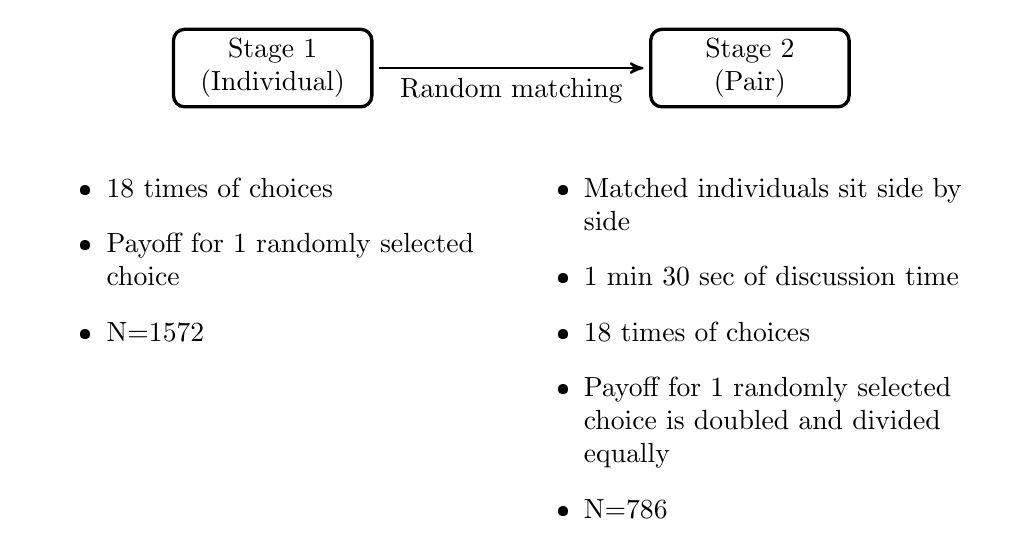
\begin{tikzpicture}[node distance=1cm, auto,]
    	\node[punkt] (stage1) {Stage 1 (Individual)} ;
    	\node[punkt, right=3.5cm of stage1] (stage2) {Stage 2 \\ (Pair)}
  		edge[pil] node[auto] {Random matching}(stage1);
    	\node[punk, below=0.3cm of stage1] (indiv) 
    	{\begin{itemize}
    	\item 18 times of choices
    	\item Payoff for 1 randomly selected choice
        \item N=1572
    	\end{itemize}} ;
       \node[punk, below=0.3cm of stage2] (col) 
       {\begin{itemize}
       \item Matched individuals sit side by side
       \item 1 min 30 sec of discussion time 
       \item 18 times of choices 
       \item Payoff for 1 randomly selected choice is doubled and divided equally 
       \item N=786
       \end{itemize}} ;
	\end{tikzpicture}
    \begin{itemize}
    \item No feedback is given during the experiment and subjects are informed only the  sum of payoff from stage 1 and 2 after all the process
    \item The experiment is computerized using O-tree
    \hyperlink{ex}{\beamergotobutton{ex}}
    \end{itemize}
	\end{center}
	\end{frame}
    
        \begin{frame}\frametitle{Example of Individual-pair Relative Demand Curve}
    \label{ex}
    \begin{figure}       
        \includegraphics[width=270pt,height=180pt]{img/relconsumption284.png}
       \end{figure}   
    \hyperlink{Design}{\beamerreturnbutton{Design}}
    \hyperlink{CCEI}{\beamerreturnbutton{CCEI}}
    \hyperlink{alpha}{\beamerreturnbutton{alpha}}   
    \hyperlink{Risk}{\beamerreturnbutton{Risk}}
    \end{frame}
    
     \begin{frame}\frametitle{Extension: Testing Rationality}
     \label{CCEI}
        \begin{block}{Generalized Axiom of Revealed Preference (GARP)}
         If $x^t$ is revealed preferred to $x^s$, then $x^s$ is not strictly revealed preferred to $x^t$ (\(p^sx^s \leq p^sx^t\))
        \end{block}
        \begin{block}{Afriat's theorem (Afriat (1967))}
		Observed choice data satisfy the GARP if and only if there exist a increasing, continuous and concave utility function that rationalize the observed choice. 
		\end{block}
        \begin{block}{Critical Cost Efficiency Index (CCEI(Afriat (1972)))}
		CCEI is the largest number \(e\in [0, 1]\) such that if $     e(p^1x^1)\geq p^1x^2, e(p^2x^2) \geq p^2x^3, ... , e(p^{n-1}x^{n-1}) \geq p^{n-1}x^n$, then $e(p^nx^n) \leq p^nx^1 $ \hyperlink{fig}{\beamergotobutton{fig}}       
        \end{block}
        In our data, 62.6\%(50.7\%) of individuals' CCEI are equal to or greater than 0.90(0.95). On pairs, the percentage is 70.4\%(60\%) \\
        \hyperlink{ex}{\beamergotobutton{ex}}         
    \end{frame}
        
        \begin{frame} \frametitle{Extension: Collective Rationality?}
        \begin{itemize}
        \item Many of former studies apply revealed preference approach to individual choice data (Battalio et al. (1973), Sippel (1997), Andreoni and Miller (2002), Harbaugh et al. (2001), Choi et al. (2014))
        \item We use this approach in testing collective rationality, which means consistency within choices matters. 
        \item It equals to testing whether group choices can be represented as an rational individual's decision (Representative Agent Model).
        \item Having different decision making ability and preference, individuals within collective have to compromise and reach a consensus to construct a common goal.
        \end{itemize}
        \end{frame}
        
        \begin{frame} \frametitle{Extension: Individual Rationality Leads to Group Rationality}
        \begin{figure}
        \includegraphics[width=200pt,height=150pt]{img/Figure4.png}
        \caption{CDFs of Collective CCEI by Individual Rationality}
		\end{figure}
        \begin{small}
        \begin{itemize}
        \item 57.8\%, 64.9\% and 80.9\% of neither,either,both-rational pairs have CCEI$\geq$ 0.9\footnote{This result is robust to the cutoff of CCEI to 0.95 and 0.99.}
        \end{itemize}
        \end{small}
	\end{frame}

	\begin{frame}\frametitle{Preference Aggregation: Measuring Risk Attitude}
    We use both non-parametric and parametric way in measuring risk attitude
    \begin{enumerate}
    \item Non-parametric way
    \begin{itemize}
    \item Can include all subjects to the analysis
    \item Limited information
    \end{itemize}
    \item Parametric way
    \begin{itemize}
    \item Rich information (Probability weighting, risk premium, utility curvature)
    \item Only applicable to choice data of which CCEI is high enough to assume a utility function
    \end{itemize}
    \end{enumerate}
    \end{frame}
    
      \begin{frame}\frametitle{Preference Aggregation: Measuring Risk Attitude}
    \label{Risk}
    \begin{block}{Non-parametric risk attitude\(:= \sum_{j=1}^{18} \frac{x_{cheaper}}{x_1+x_2} \in [0.5,1] \)}    
    \begin{itemize}
        \item If risk neutral, one puts all money to cheaper good (same probability)
        \item If extremely risk averse, one equalizes payoff in each state 
        \item Mean(sd) of individual/collective game=0.67(0.13)/0.70(0.13)
        \end{itemize}  
    \end{block}
    \hyperlink{ex}{\beamergotobutton{ex}}    \hyperlink{decision}{\beamergotobutton{decision}}
   \end{frame}
        
       \begin{frame}\frametitle{Preference Aggregation: Measuring Risk attitude}    
    \label{alpha}
    \begin{block}{Parametric risk attitude: Probability Weighting}
        \begin{itemize}   
         \item $U(x_{min},x_{max})=\alpha{u(x_{min})}+(1-\alpha)u(x_{max})$ (Gul (1991))
     	\item  If $\alpha=\frac{1}{2}$, \textbf{Expected Utility Form (EUT)}. If $\alpha>\frac{1}{2}$, then one said to show disappointment aversion; $\alpha<\frac{1}{2}$, elation loving. Altogether, \textbf{Rank Dependent Utility Form (RDU)} 
        \item In our data, 20.2\%, 29.3\% of individuals and pairs follow RDU, respectively.\footnote{One's utility follows EUT if $0.5 \in [\hat{\alpha}-1.96\hat{\sigma},\hat{\alpha}+1.96\hat{\sigma}]$, where $\hat{\sigma}$ is bootstrapped standard error}
        \item In addition, we assume CARA utility function which takes the specific form $u(x)=-\frac{exp(-\rho x)}{\rho}$
        \end{itemize}
    \end{block}    
    \hyperlink{RDU}{\beamergotobutton{RDU}} \hyperlink{ex}{\beamergotobutton{ex}}
    \hyperlink{estimation}{\beamerreturnbutton{est}}
    \end{frame}
 
        \begin{frame}\frametitle{Preference Aggregation: Measuring Risk attitude}    
 \begin{block}{Parametric risk attitude: Risk Premium}
        \begin{itemize}   
         \item $U(x_{min},x_{max})=\alpha{u(x_{min})}+(1-\alpha)u(x_{max})$
     	 \item Risk premium $r(h=1)$: $U(w(1-r))=\alpha{U(w(1-h))}+(1-\alpha)U(w(1+h))$
        \item Mean(sd) of individual/collective game=0.15(0.96)/0.31(1.22)\footnote{CARA function assumed} \hyperlink{ex}{\beamergotobutton{ex}}
        \end{itemize}
    \end{block}    
    \end{frame}
    
     \begin{frame}\frametitle{Preference Type Aggregation: Result}
    \begin{table}[]
\centering
\begin{tabular}{@{}ccllll@{}}
\toprule 
\multicolumn{2}{l}{Individual} & \multicolumn{1}{c}{Both EUT} & \multicolumn{1}{c}{EUT and RDU} & \multicolumn{1}{c}{Both RDU} & Total \\ \cmidrule(r){1-6}
\multirow{2}{*}{Collective} & EUT & 74.5(117) & 59.1(52) & 50.0(7) & 68.0(176) \\
	& RDU & 25.5(40) & 40.1(36) & 50.0(7) & 32.1(83) \\
	& Total & 100(157) & 100(88) & 100(14) & 100(259) \\ \bottomrule
    \multicolumn{6}{l}{\footnotesize{EUT is defined as 0.5$\in$ 95\% CI of $\alpha$, N for each case in parenthesis}} \\
     \multicolumn{6}{l}{\footnotesize{Only includes pairs with both individuals' and collective CCEI>=0.9}}
\end{tabular}
\caption{Percentage of RDU Type of Pairs by Individual Type}
\end{table}
    \end{frame}
    
    \begin{frame}\frametitle{Preference Attitude Aggregation: Result}
    \begin{figure}
        \includegraphics[width=200pt,height=150pt]{img/Figure5.png}
        \caption{CDFs of Collective Risk Preference by Individual Risk Attitude}
		\end{figure}
        \begin{itemize}
        \item 20.7\%, 49.2\% and 73.7\% of neither,either,both-risk averse pairs are more risk averse than the mean
        \end{itemize}
    \end{frame}
   
       \begin{frame}\frametitle{Preference Attitude Aggregation: Result}
    \begin{figure}
        \includegraphics[width=200pt,height=150pt]{img/Figure6.png}
        \caption{CDFs of Collective Risk Premium by Individual Risk Attitude}
		\end{figure}
    \end{frame}
    
        \begin{frame}
    \begin{footnotesize}
    \begin{table}[]
\centering
\begin{tabular}{@{}lcccc@{}}
\toprule
Dependent Var. & \multicolumn{2}{c}{Collective Risk Preference} & \multicolumn{2}{c}{Collective Risk Premium} \\ 
 & (1) & (2) & (3) & (4) \\ \midrule
Ave.(Individual RP) & 0.811*** & 0.796*** &  &  \\
 & (0.060) & (0.062) &  &  \\
Dist.(Individual RPs) & 0.017 & 0.002 &  &  \\
 & (0.052) & (0.054) &  &  \\
Ave.(Individual Premium) &  &  & 0.277** & 0.242* \\
 &  &  & (0.127) & (0.135) \\
Dist.(Individual Premium) &  &  & 0.152* & 0.170** \\
 &  &  & (0.080) & (0.081) \\
Non coed &  & 0.017 &  & 0.064 \\
 &  & (0.010) &  & (0.091) \\
Two boys &  & 0.020 &  & 0.233 \\
 &  & (0.023) &  & (0.143) \\
Two girls &  & -0.021 &  & 0.296* \\
 &  & (0.015) &  & (0.167) \\
Math Score & No & Yes & No & Yes \\
Network Characteristics & No & Yes & No & Yes \\
TIPI Scores & No & Yes & No & Yes \\
Constant & 0.151*** & 0.065 & 0.157*** & 0.709 \\
 & (0.037) & (0.053) & (0.041) & (0.519) \\
Observations & 786 & 771 & 320 & 314 \\
R-squared & 0.318 & 0.341 & 0.068 & 0.133 \\ \midrule
\multicolumn{5}{l}{\begin{tabular}[c]{@{}l@{}}Notes: 1) *** p\textless0.01, **,p\textless0.05, * p\textless0.1,  2) Standard errors are clustered at class level\\         3) Network characteristics include mean, distance of indegree and  outdegree. \\ Dyadic relationship is also controlled., 4) TIPI scores consist of outgoing, \\ openness to experience, conscientiousness, emotional stability and agreeableness.\end{tabular}}
\end{tabular}
\end{table}
\end{footnotesize}
    \end{frame}
    
	 \begin{frame}\frametitle{Pareto Efficiency: Measure}
       	 \begin{block}{Pareto Efficiency:}
         A pair's choice $X_c$ is \textbf{Pareto efficient} if and only if it is between $X^*_1=argmax_{(x_1,x_2)}\hat{U}_1(x_1,x_2)$ and $X^*_2=argmax_{(x_1,x_2)}\hat{U}_2(x_1,x_2)$
         \end{block}
\begin{center}        
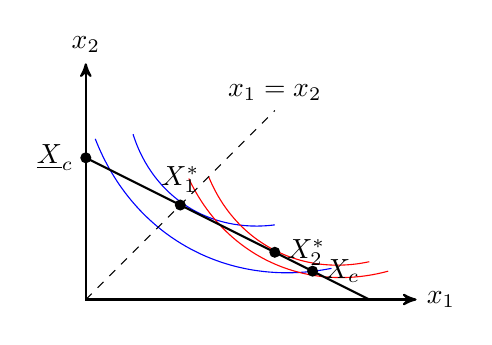
\begin{tikzpicture}[
        scale=1.2,
        IS/.style={black, thick},
        LM/.style={black, dashed},
        i1/.style={blue},
        i2/.style={red},
        axis/.style={thick, ->, >=stealth', line join=miter},
        every node/.style={color=black},
        dot/.style={circle,fill=black,minimum size=4pt,inner sep=0pt,
            outer sep=-1pt},
    ]
    % axis
    \draw[axis,<->] (3.5,0) node(xline)[right] {$x_1$} -|
                    (0,2.5) node(yline)[above] {$x_2$};
    % IS-LM diagram
    \draw[i1] (0.5,1.75) to [bend right=40] coordinate[pos=0.1] (l_i) (2,0.79) ;
    \draw[i1] (0.1,1.7) to [bend right=40] coordinate[pos=0.1] (l_i) (2.6,0.33) ;
    \draw[i2] (1.3,1.3) to [bend right=40] coordinate[pos=0.1] (l_i) (3,0.4) ;
    \draw[i2] (1.09,1.28) to [bend right=40] coordinate[pos=0.1] (l_i) (3.2,0.3) ;
    \draw[LM] (0,0) coordinate (LM_1) -- (2,2) coordinate (LM_2) node[above] {$x_1=x_2$};
    \draw[IS] (0,1.5) coordinate (IS_1) -- (3,0) coordinate (IS_2) ;

    %Intersection is calculated "manually" since Tikz does not offer
    %intersection calculation for parabolas
    \node[dot,label=above:$X^*_1$] at (1,1) (int1) {};
	\node[dot,label=right:$X^*_2$] at (2,0.5) (int1) {};
	\node[dot,label=right:$X_c$] at (2.4,0.3) (int1) {};
    \node[dot,label=left:$\underline{X}_c$] at (0,1.5) (int1) {};    
    \end{tikzpicture}
\end{center}
    \end{frame}
    
	 \begin{frame}\frametitle{Pareto Efficiency: Continuous Measure}
       	 \begin{block}{Utility Loss from Pareto Inefficient Choice:=}
         \begin{center} 
         \begin{equation}
         \frac{1}{18}\Sigma_{j=1}^{18}\frac{1}{2}\Sigma_{i=1}^2\frac{u_i(\bar{X}_{cj})-u_i(X_{cj})}{u_i(\bar{X}_{cj})-u_i(\underline{X}_{ij})} \in[0,1]
          \end{equation} 
          \end{center}
         where $X_c$: collective choice, $\underline{X}$: worst choice on the budget line. $j$ denote the sequence of budget lines and $i$ individuals. Finally, $\bar{X}=argmin(dist(X_c,X)), X\in \lbrace x|u_i(X)>=u_i(X_c) \rbrace$ with strict inequality for one $i$. If such $X$ does not exist, $\bar{X}=X_c$
         \end{block}
    \end{frame}
    
    \begin{frame}\frametitle{Pareto Efficiency: Results}
    \begin{figure}       
     \includegraphics[width=200pt,height=150pt]{img/Figure8.png}
     \caption{Distribution of the Utility Loss from Pareto Inefficiency By Pairs}
		\end{figure}   
        \begin{itemize}
        \item The mean(sd) of utility loss is 0.09(0.12) when only including pairs with both individuals' CCEI>0.9 
        \end{itemize}
    \end{frame}
    
    \begin{frame}\frametitle{Pareto Efficiency: Results}
    \begin{figure}       
     \includegraphics[width=200pt,height=150pt]{img/Figure9.png}
               \caption{CDFs of the Utility Loss from Pareto Inefficient Choices by Collective Rationality}
		\end{figure}   
        \begin{itemize}
        \item Mean of utility loss for pairs with collective CCEI>0.08 is 0.15. For CCEI<0.9, it is 0.15. This difference is statistically significant at 1\% significance level
        \end{itemize}
    \end{frame}
    
	\begin{frame}
    \begin{footnotesize}
    \begin{table}[]
\centering
\begin{tabular}{@{}lcccc@{}}
\toprule
Dependent Var. & \multicolumn{4}{c}{Utility Loss from Collective Decision} \\ \midrule
 & (1) & (2) & (3) & (4) \\
Collective CCEI & -0.369*** & -0.390*** & -0.365*** & -0.387*** \\
 & (0.067) & (0.058) & (0.066) & (0.056) \\
Ave.(Individual RP) & 0.093 & 0.099 &  &  \\
 & (0.114) & (0.101) &  &  \\
Dist.(Individual RP) & -0.139* & -0.129** &  &  \\
 & (0.072) & (0.062) &  &  \\
Ave.(Individual Premium) &  &  & -0.027 & -0.027* \\
 &  &  & (0.018) & (0.016) \\
Dist.(Individual Premium) &  &  & -0.002 & -0.006 \\
 &  &  & (0.010) & (0.009) \\
Non Coed &  & -0.011 &  & -0.009 \\
 &  & (0.023) &  & (0.023) \\
Two Boys &  & 0.065* &  & 0.072* \\
 &  & (0.039) &  & (0.039) \\
Two Girls &  & -0.018 &  & -0.014 \\
 &  & (0.027) &  & (0.026) \\
Constant & 0.413*** & 0.352** & 0.458*** & 0.400*** \\
 & (0.095) & (0.137) & (0.063) & (0.136) \\
Observations & 320 & 314 & 320 & 314 \\
R-squared & 0.075 & 0.220 & 0.070 & 0.219 \\ \midrule
\multicolumn{5}{l}{\begin{tabular}[c]{@{}l@{}}Notes: 1) *** p\textless0.01, **,p\textless0.05, * p\textless0.1,  2) Standard errors are clustered at class level\\         3) Network characteristics include mean, distance of indegree and  outdegree. \\ Dyadic relationship is also controlled., 4) TIPI scores consist of outgoing, \\ openness to experience, conscientiousness, emotional stability and agreeableness.\end{tabular}}
\end{tabular}
\end{table}
\end{footnotesize}
    \end{frame}
    
    
    \begin{frame}\frametitle{Conclusion}
    We study fundamental questions on group decision. And the results show
    \begin{block}{Extension (of Rationality)}
    If each individuals' choices are more consistent with utility maximization model, group's choice tend to also be
    \end{block}
    \begin{block}{Preference Aggregation}
    Individuals' risk attitude is strongly reflected into that of group
    \end{block}
    \begin{block}{Pareto Efficiency}
    There exists much heterogeneity in whether a group's choice is Pareto efficient or not and how much the loss is from inefficient choice. However, we find that the more rational a group is, the more efficient the group's choice is
    \end{block}
    \end{frame}
    
 
    
 	\begin{frame}\frametitle{Previous Literature}
    \begin{scriptsize}
    \begin{table}[]
\centering
\begin{tabular}{@{}lll@{}}
\toprule
Groups & Main Focus & Literature \\ \midrule
\begin{tabular}[c]{@{}l@{}}Experimental studies \\ on the  comparison between \\ individual and group   decision\end{tabular} & \begin{tabular}[c]{@{}l@{}}Which one is closer \\ to the theoretical prediction\end{tabular} & \begin{tabular}[c]{@{}l@{}}Bone et al. (1999), \\ Cason and Mui(1997), \\ Charness  et al. (2007), \\ Charness and Sutter (2012), \\ Cooper and Kagel (2005), \\ Carbone   et al. (2016), \\ Kerr at el. (1996),  Kugler et al. (2012), \\ Masclet et al.(2009), \\ Shupp and Williams (2008), \\ Sutter (2009)\end{tabular} \\ \hline
\begin{tabular}[c]{@{}l@{}}Experimental studies \\ on preference aggregation \end{tabular} & \begin{tabular}[c]{@{}l@{}} How risk attitude/ \\ time preference is aggregated \end{tabular} & \begin{tabular}[c]{@{}l@{}}Abdellaoui et al. (2010), \\ Baillon et al. (2016),\\  Bateman and Munro (2005),\\   Palma et al. (2010), \\ Lee at el. (2012)\end{tabular}\\ \hline
\begin{tabular}[c]{@{}l@{}}Empirical studies \\ on household resource  allocation\end{tabular} & \begin{tabular}[c]{@{}l@{}}Test representative agent \\ model \\   Factors for bargaining power\end{tabular} & \begin{tabular}[c]{@{}l@{}}Browning and Chiappori (1998), \\ Chiappori and  Ekeland (2011), \\ Friedberg and Webb (2006), \\ Bourguignon et al. (2009)\end{tabular} \\ \hline
Theoretical studies \\ on preference aggregation & \begin{tabular}[c]{@{}l@{}}Representative agent models\\   Impossibility theorem\end{tabular} & Arrow, Jackson and Yariv (2014)  \\ \bottomrule
\end{tabular}
\end{table}
\end{scriptsize}
    \end{frame}
    
            \begin{frame} \frametitle{Extension: Measure of Rationality}
        \label{fig}
        \begin{figure}
        \includegraphics[width=200pt,height=150pt]{img/fig_ccei.png}
		\end{figure}
        \hyperlink{CCEI}{\beamergotobutton{CCEI}}
        \end{frame}
        
        \begin{frame}\frametitle{Example of Individual-pair Relative Demand Curve}
    \begin{figure}       
        \includegraphics[width=270pt,height=180pt]{img/relconsumption623.png}
       \end{figure}   
    \hyperlink{Design}{\beamerreturnbutton{Design}}
    \hyperlink{CCEI}{\beamerreturnbutton{CCEI}}
    \hyperlink{alpha}{\beamerreturnbutton{alpha}}   
    \hyperlink{Risk}{\beamerreturnbutton{Risk}}
    \end{frame}
    
  	\begin{frame}\frametitle{EUT and RDU}
        \label{RDU}
        \begin{figure}       
        \includegraphics[width=270pt,height=180pt]{img/indifcurve.png}
        \caption{Indifference Curve Depending on Probability Weighting}
		\end{figure}
        \hyperlink{alpha}{\beamerreturnbutton{alpha}}
   	\end{frame}
    
    \begin{frame}\frametitle{Estimation of Utility Function}
    \label{estimation}
    \begin{equation}
    (\hat{\alpha}, \hat{\rho})=argmin_{(\alpha,\rho)}\Sigma_{j=1}^{18}|\frac{x^*_{1j}(\alpha, \rho)}{x^*_{1j}(\alpha, \rho)+x^*_{2j}(\alpha, \rho)}-\frac{x_{1j}}{x_{1j}+x_{2j}}|
    \end{equation}
    where
    \begin{equation}
    (x^*_{1j}(\alpha, \rho),x^*_{2j}(\alpha, \rho))=argmax_{(x_{1j},x_{2j})}\alpha (-\frac{exp(-\rho x_{min})}{\rho})+(1-\alpha) (-\frac{exp(-\rho x_{max})}{\rho})
    \end{equation}
    given $p_{1j}x_{1j}+p_{2j}x_{2j}=1$ and $x_{min(max)}=min(max)(x_{1j},x_{2j})$
    \end{frame}
    
    \end{document}
    
    